% Define document class
\documentclass[twocolumn]{aastex631}

\newcommand{\flatiron}{\affiliation{Center for Computational Astrophysics, Flatiron Institute, New York, NY 10010, USA}}
\usepackage{amsmath}
\usepackage{amssymb}
\usepackage{bm}
\usepackage{xcolor}
\definecolor{rb4}{HTML}{27408B}
\newcommand{\kw}[1]{{\color{rb4}[KW: #1 ]}}
% Begin!
\begin{document}
\title{Backpropagating Gravitational wave events}

\pacs{}

\author{Kaze W. K. Wong} 
\email{kwong@flatironinstitute.org}
\flatiron


\date{\today}

\begin{abstract}
In this
\end{abstract}

%\maketitle

\section{Introduction}

As gravitational-wave (GW) detectors sensitivity improve, the rapid increase of GW detectors shifts out 
\kw{think about the first sentence.}

A very common way to study the origin of detected GW events is through forward modelling of GW progenitor.
Forward modelling of a binary system start with a set of initial binary parameters,
then evolve it according to the physics of interest until some stopping criteria is met.
This usually mean either a merger event or the binary system stays stable for a Hubble time.

While forward modelling has been the canonical pathway to simulate binary systems and compare to GW observation,
it is not necessarily the most efficient way to constraint the underlying physical model.
Most of the systems do not end in a merger, and the systems ending up as merger events do not necessarily agree with the observation.
This means if we want to evolve a binary to match the observation by pure trial and error, a large fraction of computation will be wasted in trying initial binary configurations that are not related to the observation.
To alleviate this inefficiency, the community often takes a population approach --- instead of trying to match binary systems to observations event by event,
one can draw systems from an initial population, forward model each member in that population then match it to the observed population properties.
However, this approach is essentially trading one inefficiency with another, since we still need to choose an initial distribution of binary parameters.
For relatively well-known source properties such as initial masses this is less of a problem,
but the distribution of some less well-studied properties such as common envelope efficiency is often heuristically chosen to be some simple distribution such as a delta function at some value, i.e. a fixed value for the entire population.
This is a problem when the target of a study is to understand these less studied parameters, since one either need to justify their choice of distribution with other independent studies,
or they should vary the family of distributions.
In general, it is unclear how one can cover all possible distribution that may agree with the observation in generating a suite of simulations.
The problem worsen as we increase the dimensionality of the parameter space.

Indeed, one of the most common skepticism population synthesis studies receives is a simulations set usually only cover a small subdomain of the entire parameter space,
i.e. only vary a number of hyper-parameters while holding all others fixed to some "default" values.
Even with recently development on using emulators to speed up the simulation process, training the emulators also require a decent amount of samples in the parameter space of interest.
For example, say we want to emulate a model with 10 parameters, this simplest option for constructing a bank of simulations for training is to lay down a grid. Along each axis we put the barely minimum of $2$ simulations, this would still require $1024$ simulations.
The fastest kind of population synthesis simulation takes about an hour to complete, where longer simulations could take days.
This means even training an emulator is impossible in high dimensional space.

In this paper, instead of forward modelling a population of binary star to match the observed GW events population,
we propose a method to "backward" model each GW event to its progenitor state.
The idea is since we can compute the GW event properties of a guess by forward modelling its progenitor,
we can define the difference between the GW event properties of this guess and the observed GW event properties.
By minimizing this difference, i.e. solving a root finding problem, we can hope to recover the progenitor properties.

This paper is structured as follows: We detail our method in Sec. ~\ref{sec:method}.
In Sec. ~\ref{sec:result}, we show the results of applying our method to a number of real events.
We discuss the implications of this work and future direction in Sec. ~\ref{sec:discussion}.

\section{Method}
\label{sec:method}

We define the parameters that describe the progenitor's properties such as ZAMS masses and eccentricity as progenitor parameters $\bm{\theta'}$,
the parameters that control different physical prescriptions such as wind strength and common envelope efficiency as hyper-parameters $\bm{\lambda}$,
and random variables that affect certain stochastic process such as whether natal kick unbinds a binary as $\bm{X}$.
To avoid clutter in the following derivation,
we denote all the parameters related to mapping a particular progenitor system into a GW event collectively as evolutionary parameters $\bm{\Theta}$,
which includes $\bm{\theta'}$, $\bm{\lambda}$, and $\bm{X}$.

Once all the parameters including a particular draw of all the random variables are known,
the population synthesis code is a deterministic function that transforms the properties of the progenitors into the GW parameters.
Hence, the probability of obtaining a GW event with parameters $\bm{\theta}$ given the progenitor parameters $\bm{\theta}'$ is given by

\begin{align}
    p(\bm{\theta}|\bm{\Theta}) &= \bm{\delta}(\bm{f}(\bm{\Theta})-\bm{\theta}),
\end{align}

where $\bm{f}$ represents the population synthesis code.

While it is straightforward to write down the "forward" probability, the "backward" probability is more complicated since multiple evolutionary parameters can produce the same GW event.
Using Bayes theorem, the probability of an event with evolutionary parameters given the GW parameters can be derived as following

\begin{align}
    p(\bm{\Theta}|\bm{\theta}) &= \frac{p(\bm{\theta}|\bm{\Theta})p(\bm{\Theta})}{p(\bm{\theta})}, \nonumber \\
    &= \frac{p(\bm{\theta}|\bm{\Theta})p(\bm{\Theta})}{\int p(\bm{\theta}|\bm{\Theta}) p(\bm{\Theta}) d\bm{\Theta}}, \nonumber \\
    &= \frac{\bm{\delta}(\bm{f}(\bm{\Theta})-\bm{\theta})p(\bm{\Theta})}{\int d\bm{\theta} \bm{\delta}(f(\bm{\Theta})-\bm{\theta})p(\bm{\Theta})}.
\label{eq:backward_prob}
\end{align}

Using the result in eq.\ref{eq:backward_prob},
the probability of an event having evolutionary parameters given data can be obtained by marginalizing over the GW parameters

\begin{align}
    p(\bm{\Theta}|d) &= \int p(\bm{\Theta}|\bm{\theta}) p(\bm{\theta}|d) d\bm{\theta}\\
    &= \frac{1}{N}\sum_{i=1}^{N} p(\bm{\Theta}|\bm{\theta}_i). \label{eq:evolutionary_posterior}
\end{align}

The term $p(\bm{\theta}|d)$ is the inferred posterior probability for a particular event, which is usually presented by the LVK collaboration in the form of posterior samples.
In eq.\ref{eq:evolutionary_posterior}, we use importance sampling to turn the integration into a sum over the posterior samples.

For each posterior sample point, we can find the corresponding evolutionary parameters by solving an optimization problem that minimize the mean square difference between the GW event parameters and evolutionary parameters, i.e. 

\begin{align}
\mathcal{L}(\bm{\Theta},\bm{\theta}) = ||f(\bm{\Theta})-\bm{\theta}||^2
\label{eq:loss}
\end{align}

In principle, we should only accept solutions that exactly reproduce the LVK posterior samples in the observable space.
However, it is not feasible to achieve such condition in practice, therefore we relax the condition in eq.\ref{eq:loss} to a small acceptance threshold, in our case we picked $10^{-2}$.
To make sure we find a reasonably complete set of progenitor parameters that corresponds to the posterior sample point, we use 1000 different initial guesses in solving the optimization problem.
As long as the solution fulfill the acceptance criteria, the root is as valid as all other roots that fulfill the same acceptance criteria, regardless to its initial guess.
In other word, we have the freedom to choose the set of initial guesses however we think it might benefit the optimization.
Most of the points in the evolutionary parameter space do not produce mergers, and for systems that do not merge, we set the binary masses to be 0.
This means the gradient for systems that do not merge is 0, and the root finder would likely to get stuck in such state during the first step.\footnote{On a plateau of constant loss, the root finder performs no better than a random guess. In a high dimensional space, this means the root finder will need a long time to get close to a solution.}
Therefore, it is beneficial to put initial guesses in region of the evolutionary parameter space that does produce merger.
To construct a list of initial guesses, we evolve a set of points that we uniformly sampled from the evolutionary parameter space, then keep the points that merge within a Hubble time.
%Note that this freedom in choosing the initial guess introduces a subtlety in interpreting the posterior in the evolutionary parameter space. \kw{continue explaining}

% \kw{There is a caveat to this initialization. Imagine there are two clusters of posterior points in the evolutionary parameter space, one with N points and one with M points, do we treat each cluster as one point? Or do we give equal weight to each root? This is probably a choice at the end which matters a little bit, and depends on the prior choice, but we should clear the conceptual confusion.
% Perhaps we can put a heuristic experiment result in appendix: we randomly sample the possible root for each posterior, then use that as the result, and we do it multiple times to show the result doesn't change dramatically.
% Prior weight across posterior samples may help to alleviate the issue.}
% \kw{The most robust thing one can do is sample the prior in the evolationary parameter space, pipe it through BSE then the GW PE code. I think it is still subject to the same multiple root problem, and N-M problem will still be there.
% So in a sense, the only prior we have to take care is really the GW prior.}
% \kw{Mention how we generate the initial guesses.}

Ideally we would like to have explicit control over all evolutionary parameters.
In particular, having explicit control over random variables allows us to marginalize over their contribution, so we can focus on progenitor parameters and hyper-parameters.
However, in practice most of the population synthesis simulation code (including \texttt{COSMIC} which we use in this study.) define their random variables implicitly,
i.e. the random variables are drawn within the program, instead of being arguments of the program.
This means the function we use to evolve the binary is not a deterministic function but a stochastic function instead. 
Hence, even if the root-finding algorithm performs perfectly,
forward modelling this set of roots does not guarantee to reproduce the set of posterior samples due to randomness of the evolution function.
To assure the recovered progenitor and hyper-parameters robustly corresponds to the posterior in the GW observables space,
we forward model ("Reproject") the recovered evolutionary parameters to the observables space to check whether the reprojected posterior agrees with the posterior given by the LVK collaboration.
We use KL divergence to measure the agreement between the two posterior distributions, which is given by
\begin{align}
D_{KL}(P||Q) = \int P(\bm{x}) \log(P(\bm{x})/Q(\bm{x})) dx.
\label{eq:KLdivergence}
\end{align}

A small KL divergence means the reprojected \texttt{COSMIC} posterior is similar to the original posterior in the observable space, hence it is a viable channel for that specific event, otherwise it either means \texttt{COSMIC} can only explain part of the posterior or cannot explain the event at all.
This is completely expected since \texttt{COSMIC} comes with its own assumptions and is expected to fail in reproducing a subset of the event in GWTC3, such as event with at least one component beyond the pair instability supernova massgap.
On the other hand, the reprojection could subject to stochasticity in the evolution function we use.
Instead of reprojecting the posterior only once, we reproject the posterior multiple times with different random seeds and check whether the KL divergence varies significantly.
A varying KL divergence means this particular event is subjected to randomness in the evolution function, hence one should take extra caution in interpreting the result.


\section{Result}
\label{sec:result}

\begin{enumerate}
\item Raw posterior of successful events.
\item Trace back the event's $z_{\rm ZAMS}$.
\item Reproject to observable space
\item Evidence ratio?
\item KL divergence?
\end{enumerate}


We show a portion of the joint posterior of the progenitor parameters and hyper-parameters of GW150914 in figure \ref{fig:GW150914_posterior}.
\kw{Recover ratio of the posterior sample goes here.}

The full posterior is available in appendix \kw{Or we should w=put a link to the dataset?}


\begin{figure*}
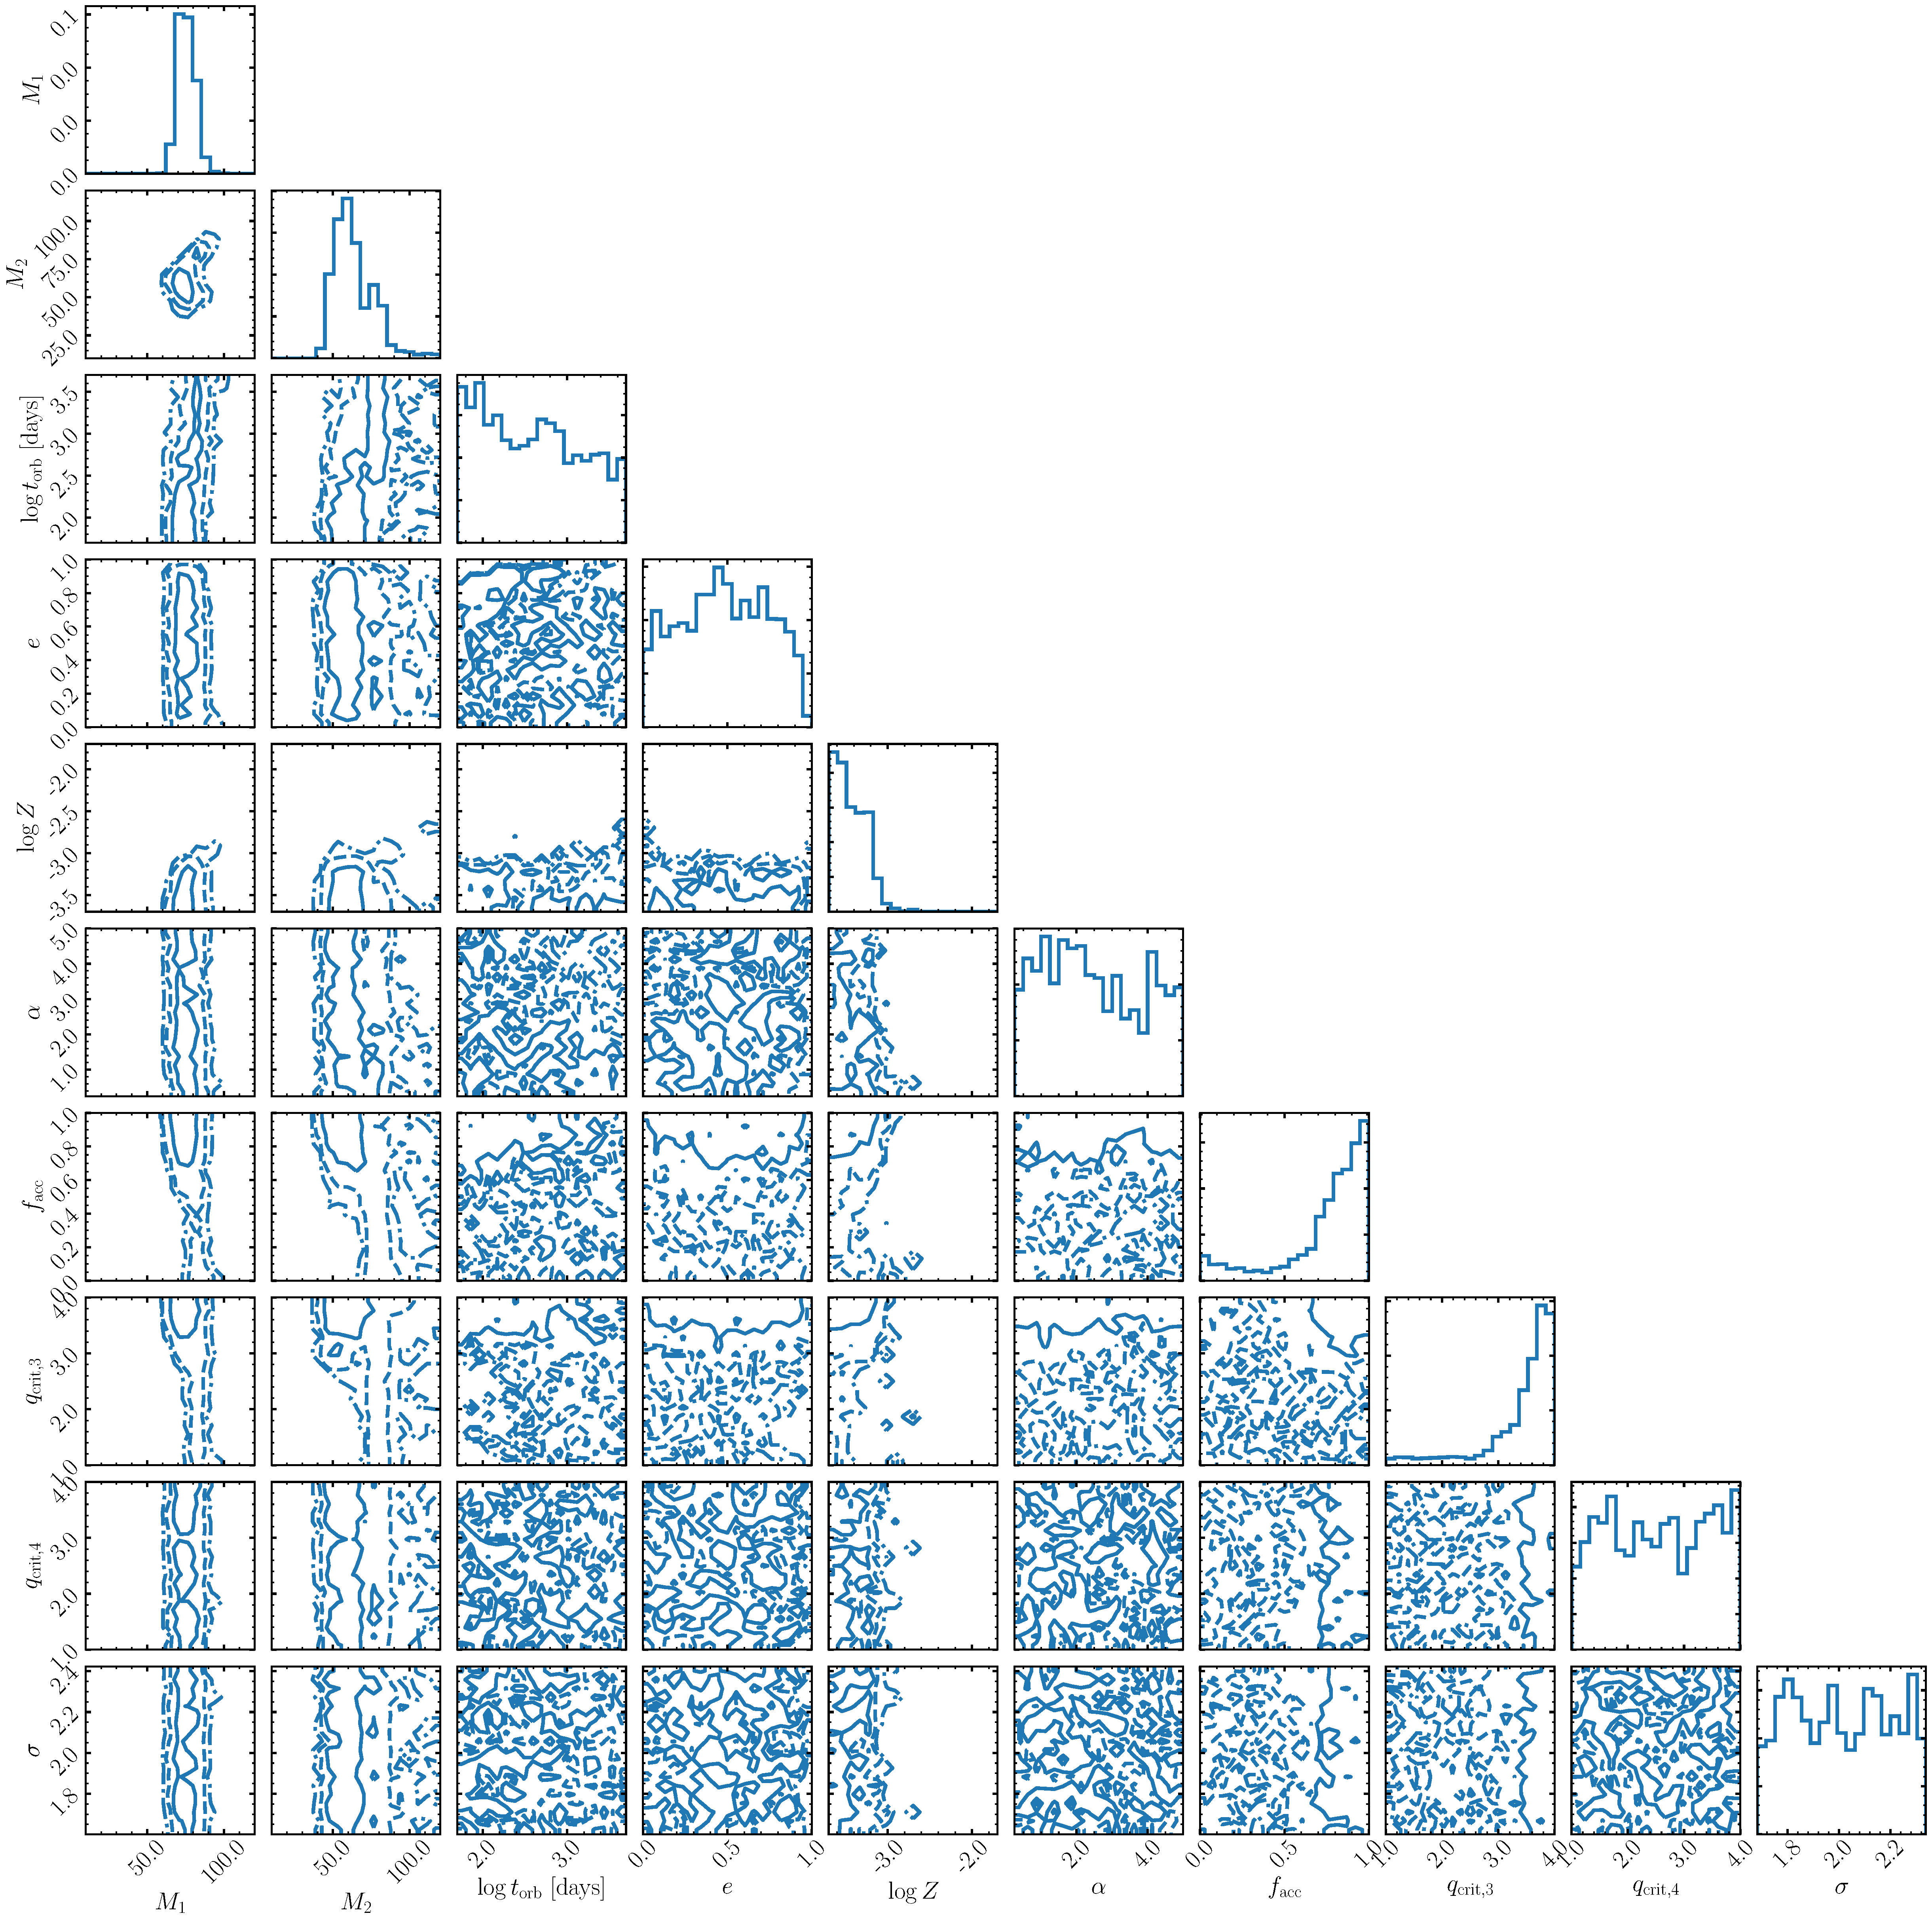
\includegraphics[width=0.98\textwidth]{static/GW150914_corner.pdf}
\caption{The posterior for GW150914 in both the progenitor parameter space and hyper-parameter space.
$M_1$ and $M_2$ are the progenitors' masses. $\log{t_{orb}}, e, \log{Z}$ are the progenitor binary's log orbital period, eccentricity and log metallicity at ZAMS.
$\alpha$ is the common envelope efficiency.
$f_{\rm acc}$ is the fraction of mass accreted during stable mass transfer.
$q_{\rm crit 3,4}$ are the ciritical mass during \kw{Katie fill in},
$\sigma$ is the mean magnitude of the Maxwellian distribution characterizing natal kick strength.
}
\label{fig:GW150914_posterior}
\end{figure*}

To check the validity of the recovered posterior, it is essential to check whether it is consistent with the original posterior in the observable space.
We reproject the recovered posterior to the observable space, and compare the KL divergence between the original posterior and the reprojected posterior.
For GW150914, the KL divergence between the reprojected posterior and the original posterior is \kw{fill later} on average.
The KL divergence stays stable for reprojecting with different random seeds.


\begin{figure}
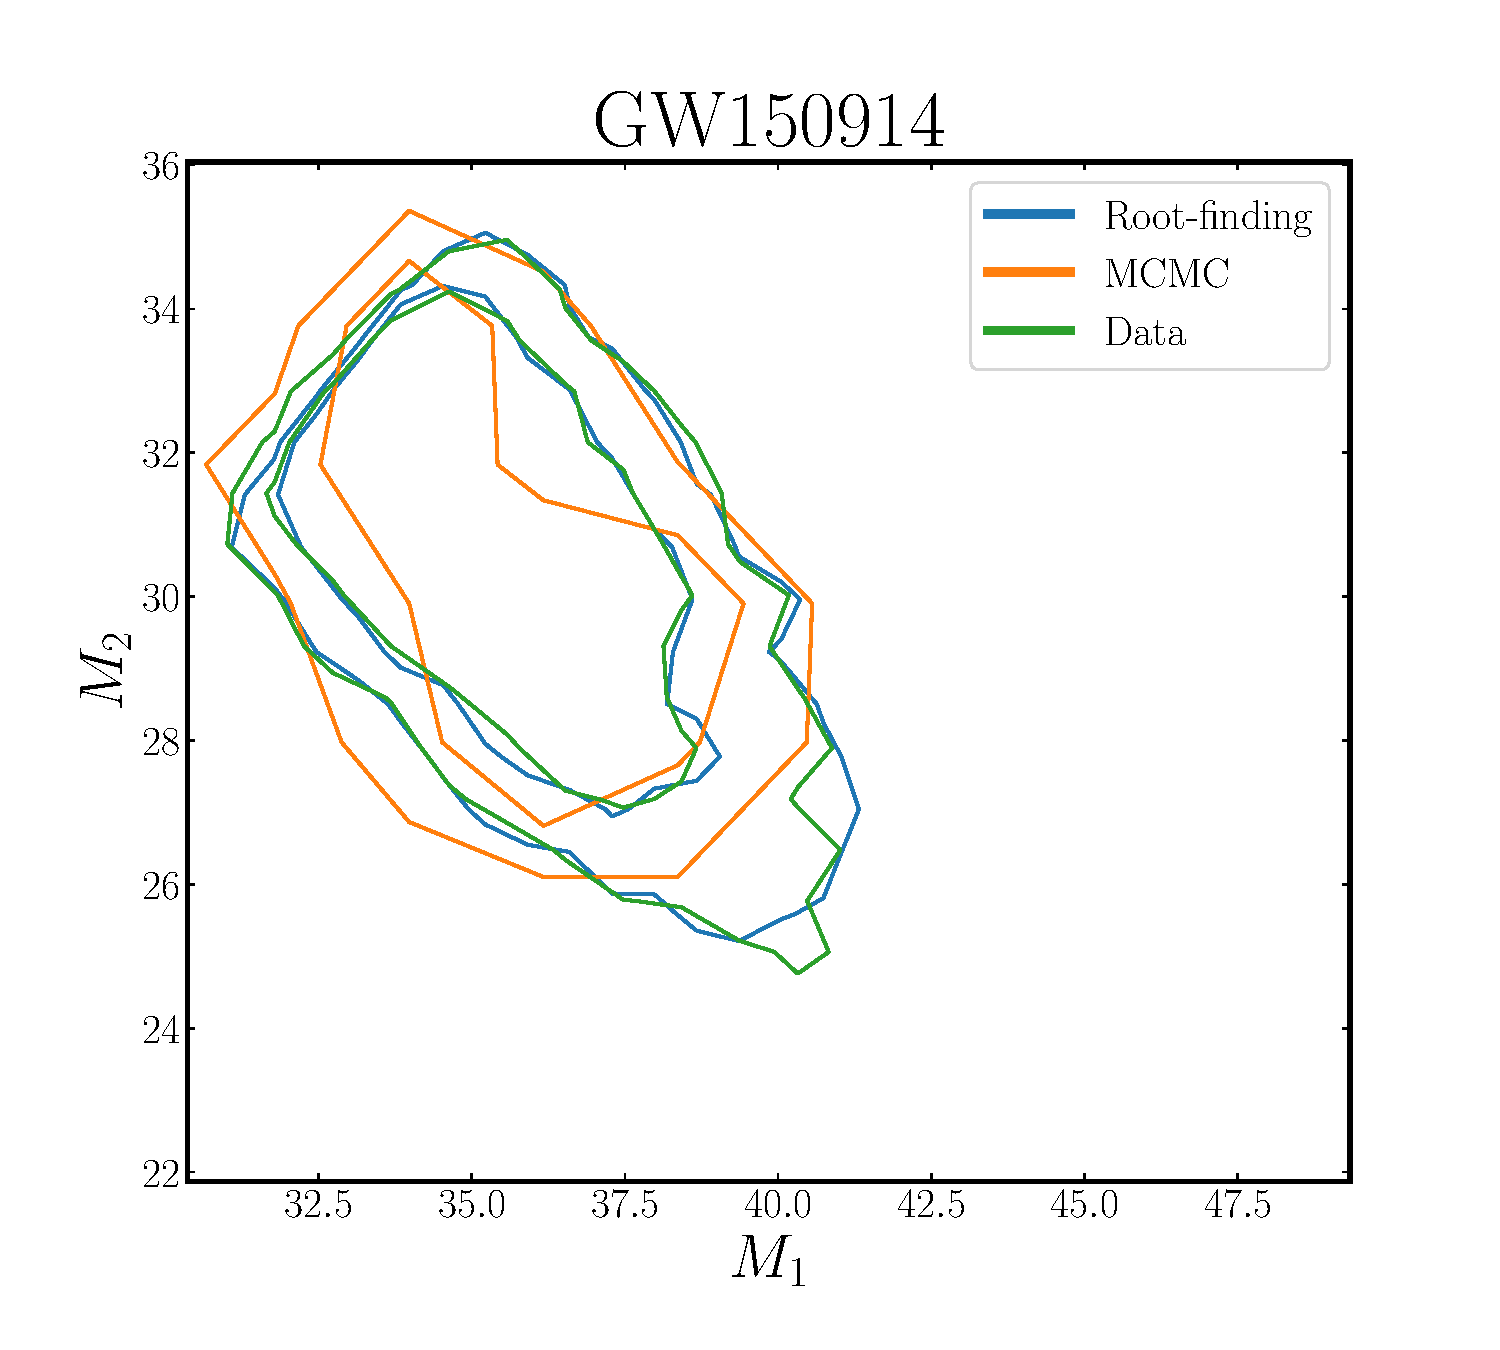
\includegraphics[width=0.49\textwidth]{static/GW150914_reprojection.pdf}
\caption{Reprojecting the posterior in evolutionary parameter space of GW150914 to observable space.
The blue contour is the posterior reprojected using the samples in the evolutionary parameter space.
The orange contour is the posterior samples from LVK that have corresponding samples in the evolutionary parameter space.
The green contour is the posterior plotted using all of LVK posterior samples.
}
\label{fig:GW150914_reprojection}
\end{figure}

We can see the reprojected posterior agrees very well with the original posterior in fig.\ref{fig:GW150914_reprojection}.
\kw{Qoute the KL divergence.}


\begin{figure}
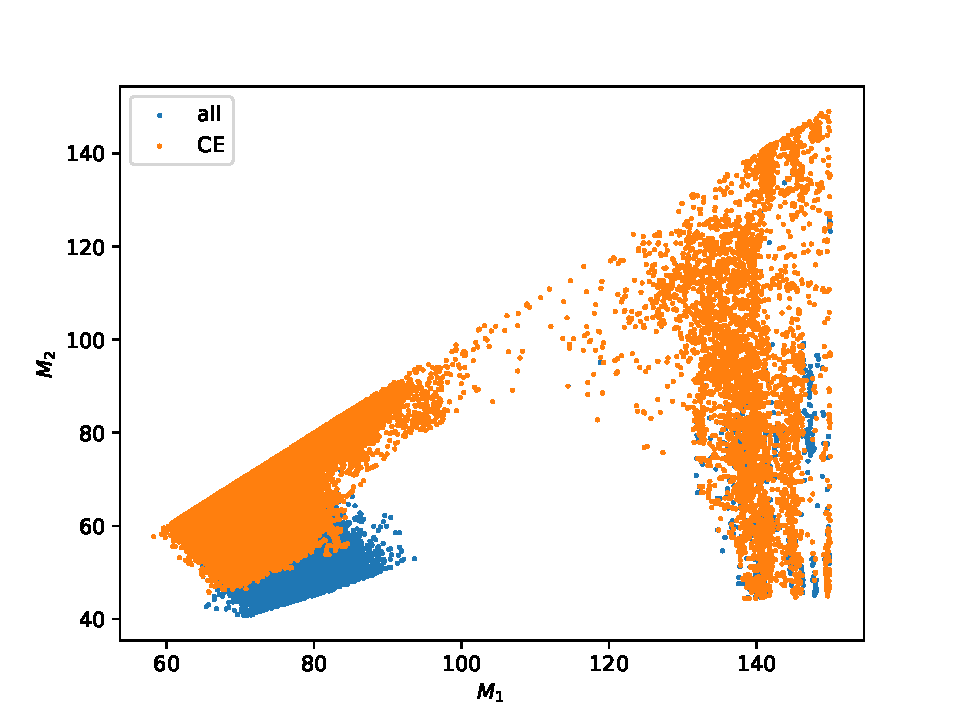
\includegraphics[width=0.49\textwidth]{static/GW150914_CE_SMT.pdf}
\caption{}
\label{fig:GW150914_CE_SMT}
\end{figure}
\kw{Add figure of stable mass transfer vs common envelope}

\begin{figure}
\caption{}
\label{fig:GW150914_M1_M2_q3}
\end{figure}


The most important point in this paper is illustrated in figure \ref{fig:GW150914_M1_M2_q3}.
We can see the posterior samples in $M_1-M_2$ space are spatially correlated with $q_3$,
this means if we fixed the value of $q_3$ instead of allowing it to jointly vary with all other parameters,
we would miss the samples that do not match the chosen value of $q_3$.
By folding in the hyper-parameters into the root-finding algorithm,
we can capture the correlation between 
\kw{Dartboard comparsion} Comparing our result with 
\kw{Add figure showing hyper-parameters are important to recovering the progenitor parameters correctly.}

\section{Discussion}
\label{sec:discussion}


We present a new pathway to understand binary evolution with GW events in this paper.
Instead of forward modelling an assumed distribution of initial binary to the observed population,
we solve a root-finding problem to find the best initial binary parameters that reproduce the posterior distribution for each event. 
The most obvious advantage our method provides is it returns the joint posterior distribution of progenitor parameters and hyper-parameters for each event.
This enables a data-driven way to study the distribution of hyper-parameters,
i.e. once we have a catalog of events, each has their own set of posterior in the hyper-parameter space,
we can employ common techniques such as hierarchical Bayesian analysis to fit a population model to the distribution of hyper-parameters,
without making specific assumptions such as fixing the hyper-parameters for all types of event.
 
In this work we showcase the power of the proposed method with two events, GW150914 and GW191129.
We show the joint posterior of the two events' progenitor parameters and hyper-parameters.
In particular, to the authors knowledge, this is the first time the correlation between progenitor parameters and hyper-parameters is shown.
Our work is not only a more efficient way to study GW events' progenitors,
but also allows the possibility of measuring the astrophysics related the binary evolution, especially in capturing the correlation between different hyper-parameters.

% Rate analysis is now just counting, like what's done in phenomenological model, instead of forward modelling.
Another perk of our method is the "rate" calculation is now independent of assumed initial condition such as a particular star formation rate model,
which is a dominant factor of uncertainty for rate prediction in the past.
Once we have pull back the GW event posterior from the observable space to the evolutionary parameter space,
we can apply the same methods we use to account for the rate in the observable space.
In the observable space, the overall rate is basically a normalization that is defined in the local universe i.e. the local merger rate. \kw{cite}
In the evolutionary parameter space, we can instead fit for the production rate of merger events at some redshift.
\kw{Talk about prior are now in post-processing instead of pre-processing.}


% Single formation channel and fundamental limitation on that.
While our method allows data-driven exploration of the hyper-parameters space for the first time, there are a number of improvements can be implemented in future studies.
In this study we use only \texttt{COSMIC} as our evolutionary function, which by design cannot explain all the events in GWTC3.
For example, event with either of the component mass larger than the PISN gap such as GW190521 cannot be explained by \texttt{COSMIC}.
Alternative channels such as dynamic formation channel will be needed to explain some subset of the events in GWTC3.
As pointed out in the literature \kw{Cite mike}, it is unlikely that all the observed events in GWTC3 can be explained by a single formation channel.
As GW detectors sensitivity increase, we expect to see more and more events that are unusual in some way.
Therefore, having a self-consistence population synthesis code that contains multiple formation channels is essential to accommodate the growing catalog of GW events.
In this paper, our main focus is to illustrate the concept of "back-propagating" GW events posterior sample in this work,
highlighting the capability of our method and motivating the community to build the next generation population synthesis code that can work with our method.
To avoid cluttering of focus, we discuss the physical implication of the result presented in this work under our specific assumption (i.e. using \texttt{COSMIC} as our evolutionary function) in a companion paper.


% Randomness paragraph
Due to the implicit definition of random variables in \texttt{COSMIC}, our evolutionary function is stochastic.
This introduces significant inefficiency in our root-finding algorithm.
The main stochasticity in \texttt{COSMIC} comes from natal kick, which significantly affect the evolution pathway of low mass events such as BNS events.
The effect of natal kick is suppressed for heavier mass events due to fallback.
This means events with the root-finding process for lighter masses are subject to stochasticity of the function,
where the root-finding process for heavier events behaves as if the evolutionary function we use are deterministic.
Indeed, we see this behavior in a couple of case studies.
For heavy event such as GW150914, the reprojected posterior agrees with the data posterior.
For light event such as GW170817, although during the root-finding process the convergence criteria is met,
the reprojected posterior does not agree with the data posterior.
Also, due to computational limitation, we only try 1000 different initial guesses per posterior sample in the root-finding process.
This means any posterior sample that has a probability of merging rarer than 1 in 1000 could be missed.
\kw{comment on the low mass ratio end.}
Obviously the problems which comes with the randomness can be alleviated by performing more tries per posterior sample,
but this is not scalable in practice.
On top of limitation in efficiency, some formation channels require explicit control of random variables by construction.
For example, in a dynamical formation scenario such as binaries that form in a globular cluster,
each binary has some probability of undergoing a multi-body encounter with another member in the cluster.
These encounter probability distributions are either studied with direct N-body simulations or semi-analytical methods.
In both cases, each member of the cluster is no longer completely independent of the other members, but coupled through the encounter probability distribution.
By studying the encounter probability distribution, we can infer the properties of the environment which the binary lives in.
This can only be done if we have explicit control over the random variables that characterize the encounter probability distribution.

% Need for selection bias to recover intrinsic distribution



% Gradient decending in the evolutionary parameter space is much more efficent than rejection sampling.
% Potential pitfall of interpreting this result.
% Need for full autodiff.

By leveraging gradient-based optimization strategy, obtaining posterior samples in the evolutionary parameter space is much more efficient than rejection sampling.
In each optimization step during the root-finding process, the current state of the guess and its gradient provide useful information about where the root might be.
In contrast to sampling algorithm, which discard the sample whenever it is not accepted.
This greatly benefit the efficiency of the root-finding process.
On the other hand, this method is not a sampling algorithm, but a coordinate transform of the posterior samples.
One should pay extra caution in interpreting the posterior samples in the evolutionary parameter space.
Since posterior samples in the observable space can in principle have multiple roots in the evolutionary parameter space,
the relatively weighting of these roots becomes ambiguous when the number of roots is large.
For example, should we consider roots that are close to each other a single root or multiple roots?
If we have two clusters of roots, the relative number of roots within each cluster would determine the relative weight of each mode.
Note that since they both map to the same observable posterior sample within the acceptance threshold, all weighting assigned are equally valid from a "matching data" standpoint.
This leave the interpretation of the posterior in the evolutionary parameter space ambiguous.
In our case, we found empirically each posterior sample may at most only correspond to a handful of roots (most of the posterior samples have a unique root.), therefore we choose to assign equal weight to each root,
and we have checked the posterior samples produced by this method for events discussed in this paper agree with direct sampling using a uniform prior.
This is due to the behavior of posterior in the evolutionary parameter space are larger determined by the posterior distribution in the observable space instead of multiple possible roots per posterior sample.
We leave a detail comparison between this method and direct sampling to future studies.

Another technical note is we use finite differencing to estimate the gradient of the objective function, which could be a significant source of error near transition points in the evolutionary parameter space.
Also, finite differencing is increasing inefficiency as we increase the dimensionality of the problem.
To improve the accuracy and efficiency in estimating the gradient of objective function, automatic differentiation is a promising feature that modeler should consider incorporating in their population synthesis code in the future.

\kw{Mention potential complimentary studies of direct sampling, and how all these suggestions are still useful regardless of whether we are doing root-finding or not.}

To summarize, we propose a novel method to recover the posterior samples in the evolutionary parameter space for each GW event.
We "back propagate" the posterior in the observable space to the evolutionary parameter space,
thus allowing us to study the correlation between progenitor parameters and hyper-parameters.
We demonstrate the capability of this method with two events, GW150914 and GW191129, while employing the binary population synthesis model \texttt{COSMIC}.
We 
We hope this letter would motivate the community to build the relevant infrastructure mentioned above,
so in the near future we can explore the full parameter space of binary evolution models with the next-generation GW detectors network.


Interpretation:
\begin{enumerate}
\item Highlight the fact that we turn hyper-parameters into parameters.
\item Discuss this is need for high dimensional exploration.
\end{enumerate}

Caveats: 
\begin{enumerate}
\item Discuss events that cannot be complete transferred backward. From BSE angle and from LIGO posterior angle. Failure mode in mass.
\item We only assume BSE
\item Caveat on marginalizing over random samples.
\item Prior need to be applied after one translate the posterior, i.e. it is a post-processing step now.
\item How next generation "Progenitor synthesis" code should be built.
\item Rate
\item Failure studies go into appendix
\end{enumerate}

\section{Acknowledgement}

\end{document}
